% ResearchShop architecture diagram for the SoftwareX paper.
% Absolute-coordinate layout with high-contrast stage bands for readability.
\documentclass[border=7pt]{standalone}
\usepackage[T1]{fontenc}
\usepackage{tikz}
\usetikzlibrary{arrows.meta,backgrounds}

\begin{document}

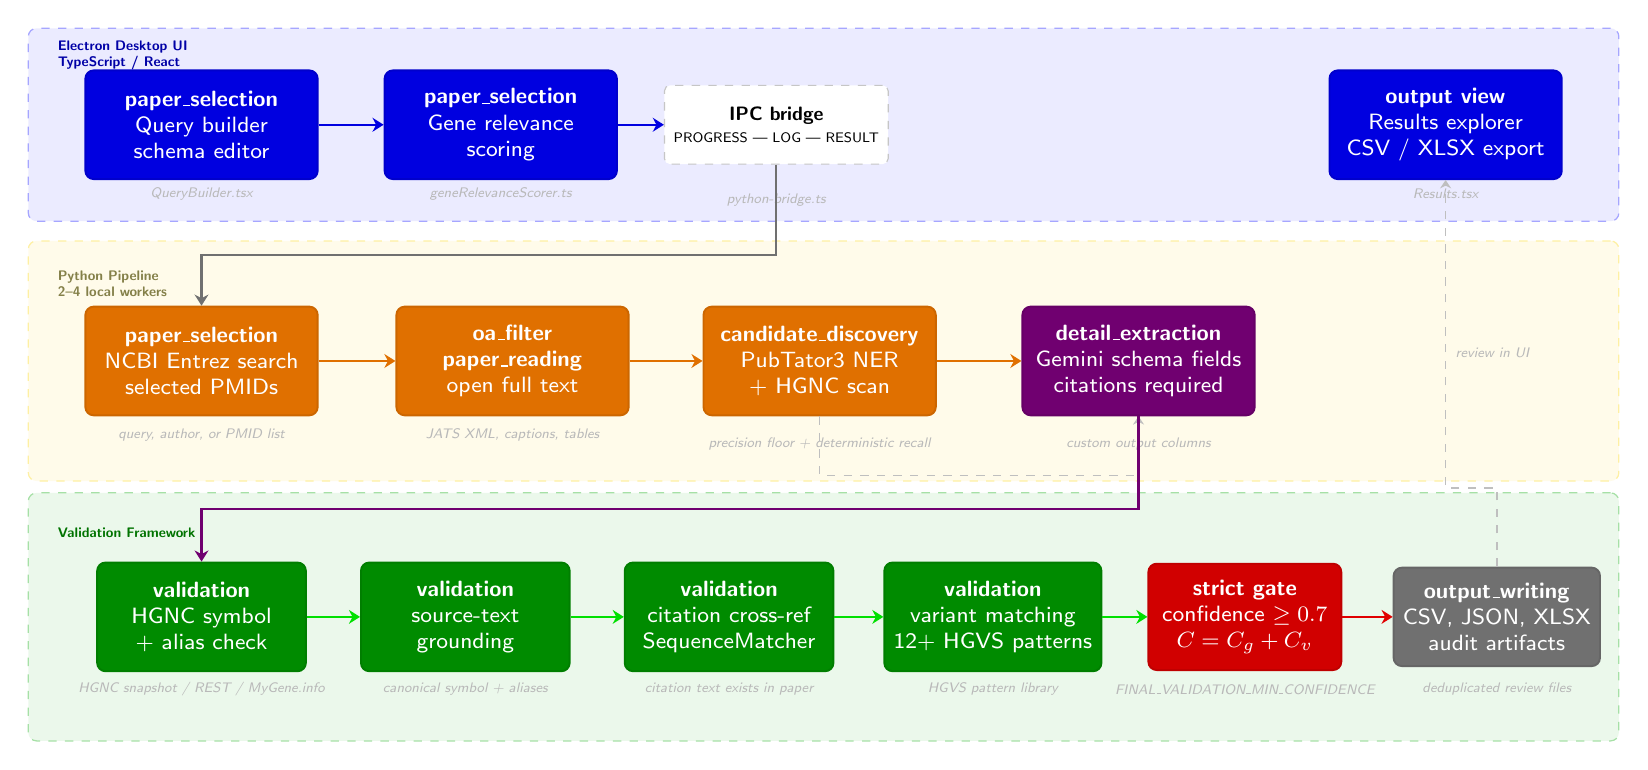
\begin{tikzpicture}[
  every node/.style={font=\sffamily},
  band/.style={
    draw=#1!35,
    fill=#1!8,
    dashed,
    rounded corners=3pt,
    line width=0.45pt
  },
  stage/.style={
    draw=#1!80!black,
    fill=#1!88!black,
    text=white,
    rounded corners=3pt,
    minimum width=2.95cm,
    minimum height=1.38cm,
    align=center,
    line width=0.7pt,
    font=\sffamily\footnotesize
  },
  stage/.default=gray,
  gate/.style={
    draw=red!75!black,
    fill=red!82!black,
    text=white,
    rounded corners=3pt,
    minimum width=2.65cm,
    minimum height=1.35cm,
    align=center,
    line width=0.7pt,
    font=\sffamily\footnotesize
  },
  aux/.style={
    draw=gray!45,
    fill=white,
    dashed,
    rounded corners=2pt,
    minimum width=2.25cm,
    minimum height=1.0cm,
    align=center,
    font=\sffamily\scriptsize
  },
  file/.style={font=\sffamily\tiny\itshape, text=gray!55, align=center},
  layer/.style={font=\sffamily\tiny\bfseries, anchor=west, align=left},
  arr/.style={-{Stealth[length=4pt,width=5pt]}, line width=0.8pt, draw=#1!88!black},
  arr/.default=gray,
  softarr/.style={-{Stealth[length=3pt,width=4pt]}, line width=0.55pt, draw=gray!50, dashed},
]

% Row backgrounds.
\begin{scope}[on background layer]
  \node[band=blue, minimum width=20.2cm, minimum height=2.45cm] at (7.9,0) {};
  \node[band=yellow!75!orange, minimum width=20.2cm, minimum height=3.05cm] at (7.9,-3.0) {};
  \node[band=green!65!black, minimum width=20.2cm, minimum height=3.15cm] at (7.9,-6.25) {};
\end{scope}

% Row 1: Electron desktop UI.
\node[layer, text=blue!65!black] at (-1.95,0.88) {Electron Desktop UI\\TypeScript / React};

\node[stage=blue] (query) at (0,0) {\textbf{paper\_selection}\\Query builder\\schema editor};
\node[stage=blue] (rank) at (3.8,0) {\textbf{paper\_selection}\\Gene relevance\\scoring};
\node[aux] (ipc) at (7.3,0) {\textbf{IPC bridge}\\{\tiny PROGRESS | LOG | RESULT}};
\node[stage=blue] (results) at (15.8,0) {\textbf{output view}\\Results explorer\\CSV / XLSX export};

\node[file] at (0,-0.88) {QueryBuilder.tsx};
\node[file] at (3.8,-0.88) {geneRelevanceScorer.ts};
\node[file] at (7.3,-0.96) {python-bridge.ts};
\node[file] at (15.8,-0.88) {Results.tsx};

\draw[arr=blue] (query) -- (rank);
\draw[arr=blue] (rank) -- (ipc);

% Row 2: Python extraction pipeline.
\node[layer, text=yellow!45!black] at (-1.95,-2.02) {Python Pipeline\\2--4 local workers};

\node[stage=orange] (select) at (0,-3.0) {\textbf{paper\_selection}\\NCBI Entrez search\\selected PMIDs};
\node[stage=orange] (read) at (3.95,-3.0) {\textbf{oa\_filter}\\\textbf{paper\_reading}\\open full text};
\node[stage=orange] (cand) at (7.85,-3.0) {\textbf{candidate\_discovery}\\PubTator3 NER\\+ HGNC scan};
\node[stage=violet] (detail) at (11.9,-3.0) {\textbf{detail\_extraction}\\Gemini schema fields\\citations required};

\node[file] at (0,-3.94) {query, author, or PMID list};
\node[file] at (3.95,-3.94) {JATS XML, captions, tables};
\node[file] at (7.85,-4.06) {precision floor + deterministic recall};
\node[file] at (11.9,-4.06) {custom output columns};

\draw[arr=gray] (ipc.south) -- ++(0,-1.15) -| (select.north);
\draw[arr=orange] (select) -- (read);
\draw[arr=orange] (read) -- (cand);
\draw[arr=orange] (cand) -- (detail);
\draw[softarr] (cand.south) -- ++(0,-0.75) -| (detail.south);

% Row 3: Validation and output.
\node[layer, text=green!45!black] at (-1.95,-5.18) {Validation Framework};

\node[stage=green!62!black, minimum width=2.65cm] (gene) at (0,-6.25) {\textbf{validation}\\HGNC symbol\\+ alias check};
\node[stage=green!62!black, minimum width=2.65cm] (ground) at (3.35,-6.25) {\textbf{validation}\\source-text\\grounding};
\node[stage=green!62!black, minimum width=2.65cm] (cite) at (6.7,-6.25) {\textbf{validation}\\citation cross-ref\\SequenceMatcher};
\node[stage=green!62!black, minimum width=2.65cm] (variant) at (10.05,-6.25) {\textbf{validation}\\variant matching\\12+ HGVS patterns};
\node[gate, minimum width=2.45cm] (strict) at (13.25,-6.25) {\textbf{strict gate}\\confidence $\geq 0.7$\\$C=C_g+C_v$};
\node[stage=gray, minimum width=2.55cm, minimum height=1.25cm] (output) at (16.45,-6.25) {\textbf{output\_writing}\\CSV, JSON, XLSX\\audit artifacts};

\node[file] at (0,-7.17) {HGNC snapshot / REST / MyGene.info};
\node[file] at (3.35,-7.17) {canonical symbol + aliases};
\node[file] at (6.7,-7.17) {citation text exists in paper};
\node[file] at (10.05,-7.17) {HGVS pattern library};
\node[file] at (13.25,-7.17) {FINAL\_VALIDATION\_MIN\_CONFIDENCE};
\node[file] at (16.45,-7.17) {deduplicated review files};

\draw[arr=violet] (detail.south) -- ++(0,-1.18) -| (gene.north);
\draw[arr=green] (gene) -- (ground);
\draw[arr=green] (ground) -- (cite);
\draw[arr=green] (cite) -- (variant);
\draw[arr=green] (variant) -- (strict);
\draw[arr=red] (strict) -- (output);
\draw[softarr] (output.north) -- ++(0,1.0) -| node[pos=0.72, right, font=\sffamily\tiny\itshape, text=gray!55]
  {review in UI} (results.south);

\end{tikzpicture}

\end{document}
